\chapter{Conclusioni e Sviluppi Futuri}
\label{cap:nomePrimoCapitoloTesi}
\lhead{\textbf{\rightmark}}

\indent{
	Questo capitolo presenta le conclusioni principali ed i possibili miglioramenti di questa ricerca/applicazione.
	In questo lavoro di tesi, si è sviluppato un sistema automatico per la diagnosi preliminare del melanoma basato sulla collaudata procedura medica ABCDE di uso comune.
	Il sistema proposto combina il metodo ABCD con le capacità di acquisizione ed elaborazione delle immagini degli smartphone per ottenere una diagnosi del melanoma rapida, conveniente, facilmente disponibile e altamente accurata.
	Il sistema prodotto include più moduli per la gestione delle varie fasi del metodo come: acquisizione di immagini, rimozione del rumore, segmentazione della lesione, estrazione di caratteristiche e, infine, classificazione (diagnosi).
	Nel metodo presentato, dopo aver acquisito l'immagine utilizzando la fotocamera del dispositivo questa viene inviata immediatamente al server per l'elaborazione, il quale pulisce l'immagine da eventuali peli o imperfezioni, mette in evidenza i bordi del nevo, ritaglia l'immagine, estrae le feature inerenti a asimmetria, centroide, diametro, bordi, 2D photometric stereo, fractal, dimensione frattale, colori e fa analizzare il nevo correttamente segmentato alla ConvNet.
	\begin{figure}[h]
		\begin{center}
			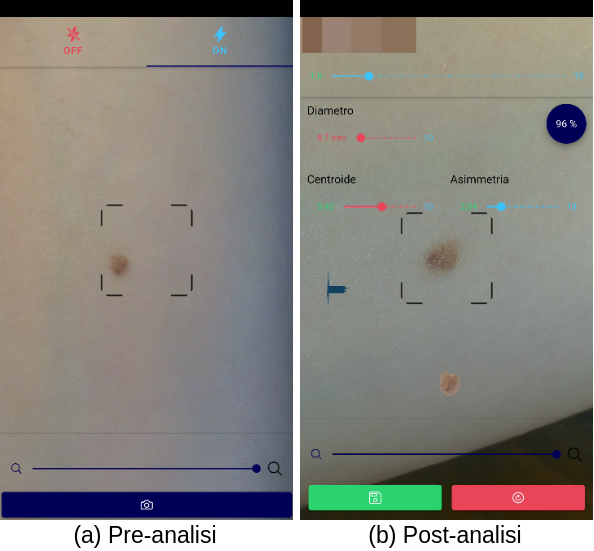
\includegraphics[scale=0.6]{figure/capitolo8/analisi.png}
		\end{center}
		\caption{Esempio dell'applicazione pre-analisi e post-analisi.}	
	\end{figure}
\newline
Gli sviluppi futuri per questo lavoro possono concentrarsi sull'aggiunta di alcune funzionalità e sul miglioramento di quelle esistenti:
\begin{itemize}
	\item Addestrare una rete neurale ad hoc per migliorare la segmentazione del nevo, che allo stato dell'arte viene effettuata con degli algoritmi che si limitano all'analisi dell'immagine ed al riconoscimento efficace dei bordi del nevo;
	\item Addestrare la rete neurale convoluzionale, che si occupa dell'analisi del melanoma, con immagini provenienti da fotocamere di smartphone;
	\item Algoritmo di riconoscimento della qualità dell'immagine sul device;
	\item Utilizzo di un sensore laser o di un riferimento sul nevo, al fine di migliorare la qualità del diametro;
	\item Sviluppare funzionalità di Evoluzione per ogni nevo e permettere al dermatologo di effettuare confronti nel tempo;
	\item Validazione dell'applicazione da parte di un dermatologo;
	\item Utilizzare le informazioni pregresse del paziente per migliorare l'analisi;
\end{itemize}
}